% arXiv v17 (Gemini round-4: exact vs bootstrap box labels, failed predictions in main text, level bound proven not measured. ../GEMINI_R4_FIXES_112626.md)
% v14 (Gemini round-2 fixes, ../GEMINI_R2_FIXES_112626.md: all 423 Table II certificates and all 2330 Table S6 declarations rechecked in Arb ball arithmetic, all pass; archive URL set unbreakable. No number changed.)
% Previous: arXiv v13 (ChatGPT final-round fixes, paper/../CHATGPT_FINAL_FIXES_112626.md: level stated for the 0.25 margin, not the 0.6 crossover; 10 of 423 certificates in ball arithmetic; bias tied to the tested smoother and bandwidths; exact-box materials go to archive v1.2. No number changed).
% Previous: arXiv v12 (Fable final readability check of v11: P(t)/q(t) notation tied together in Sec. II; main.bbl, xref_M.tex and ABSTRACT.txt regenerated to match the v11 text; no number changed).
% Previous: arXiv v11 (readability-review fixes of v10); arXiv v10, READABLE EDITION (2026-11-25). Rewritten for a reader new to the work after an endorser's feedback
% (paper/REVIEWS/ENDORSER_FULCHER_112626.md): one finding, one fix, what is new beyond Hall-Horowitz 2013 and CCF 2018.
% No stored number changed. Evidence labels, amendment history, gates, sub-variants and D_lo are in supplement.tex or the repository.
% New in v10: the exact Clopper-Pearson box for the global test (ideas/BD_exact_box_power_map/RESULTS.md).
% Build: pdflatex three times on main.tex and on supplement.tex (the .bbl files are shipped; xref_S.tex / xref_M.tex hold
% the cross-document labels, regenerate with make_xref.sh). Standard packages only; the source is ASCII.
\documentclass[aps,pre,twocolumn,superscriptaddress,nofootinbib,10pt]{revtex4-2}
\usepackage{graphicx}
\usepackage{xcolor}
\usepackage{amsmath}
\usepackage[T1]{fontenc}
\usepackage{lmodern}
\usepackage{amssymb}
\usepackage{url}
\newlabel{S-FirstPage}{{}{1}{}{}{}}
\newlabel{S-sup:bench}{{S1}{1}{}{}{}}
\newlabel{S-tab:xnames}{{S1}{2}{}{}{}}
\newlabel{S-tab:ledger}{{S2}{2}{}{}{}}
\newlabel{S-sup:env}{{S1}{2}{}{}{}}
\newlabel{S-sup:10c}{{S2}{2}{}{}{}}
\newlabel{S-sup:e7}{{S3}{3}{}{}{}}
\newlabel{S-tab:joint}{{S3}{4}{}{}{}}
\newlabel{S-tab:10c}{{S4}{4}{}{}{}}
\newlabel{S-sup:lp}{{S3}{4}{}{}{}}
\newlabel{S-sup:nodrop}{{S4}{5}{}{}{}}
\newlabel{S-tab:nodropS}{{S5}{5}{}{}{}}
\newlabel{S-sup:cp}{{S4}{6}{}{}{}}
\newlabel{S-tab:cpmap}{{S6}{7}{}{}{}}
\newlabel{S-sup:e4}{{S5}{7}{}{}{}}
\newlabel{S-sup:a13}{{S5}{7}{}{}{}}
\newlabel{S-sup:rand}{{S6}{8}{}{}{}}
\newlabel{S-sup:redteam}{{S7}{8}{}{}{}}
\newlabel{S-tab:a13b}{{S7}{9}{}{}{}}
\newlabel{S-tab:rbc}{{S8}{9}{}{}{}}
\newlabel{S-sup:prior}{{S7}{10}{}{}{}}
\newlabel{S-sup:gk}{{S8}{10}{}{}{}}
\newlabel{S-sup:soft}{{S9}{10}{}{}{}}
\newlabel{S-LastBibItem}{{9}{10}{}{}{}}
\newlabel{S-LastPage}{{}{10}{}{}{}}

\newcommand{\dt}{d_s(t)}
\newcommand{\SM}{SM}
\newcommand{\nm}[1]{\textsf{#1}}
\newcommand{\LQ}{\nm{LocQuad}}
\newcommand{\BAC}{\nm{BiasAware-CV}}
\newcommand{\BAR}{\nm{BiasAware-Rule}}
\newcommand{\BAO}{\nm{BiasAware-Oracle}}
\newcommand{\BA}{\nm{BiasAware}}
\newcommand{\SP}{\nm{StepParam}}
\newcommand{\MLP}{\nm{MonoLP}}
\newcommand{\MLJ}{\nm{MonoLP-Joint}}
\newcommand{\TL}{\nm{TwoLine}}
\newcommand{\WLS}{\nm{WLS-loglog}}
\newcommand{\RBC}{\nm{RBC}}
\newcommand{\BAS}{\nm{BiasAware-Split}}
% section references: write subsection references as III.A, not III A
\makeatletter\renewcommand\p@subsection{\thesection.}\makeatother


\begin{document}

\title{More walkers, worse error bars: bias-driven undercoverage and structural bounds for the scale-dependent spectral dimension}

\author{Adam Faust}
\affiliation{MOBLUEHQ, Inc., Long Grove, Illinois, USA}
\date{November 2026}

\begin{abstract}
The scale-dependent spectral dimension $d_s(t)$ is usually read from the log-derivative of a random-walk return probability estimated from noisy data. We ask whether the error bands drawn around such curves can be trusted, and score nominal 95\% bands against exact curves for lazy walks on tori and products of cycles. The main finding is that a standard smoothing band becomes less reliable as data are added: a local-quadratic band with a cross-validated bandwidth covered the exact curve through a dimensional crossover in 40.4\%, 19.6\% and 3.6\% of answered datasets at 8, 32 and 128 walkers per node, an ordering predicted in advance and repeated in a replication and a holdout. The cause is smoothing bias. The same bands covered their own smoothed target in 93.0--94.7\% of datasets, and, for the smoother and bandwidths tested, the bias is set by the time grid, which more walkers do not refine. Robust bias correction, the standard remedy, reduced the decline without removing it (83.5\%, 66.3\% and 47.5\% on six graphs). The constructive result uses a fact that smoothing theory does not: the return probability of a lazy walk is exactly a positive mixture of decaying exponentials. Linear programming over all such mixtures that fit a confidence box bounds $d_s(t)$ with no bandwidth or smoothness constant (98.8\% crossover coverage on a discretised measure, with a nominal box), and gives a global test that declares a crossover when no admissible mixture avoids one. With an exact Clopper--Pearson box a false declaration of a drop above 0.25 has probability at most 5\% at any sample size, a proven bound that the runs illustrate rather than measure. The test declared a two-dimensional crossover in 1, 85 and 100 of 100 datasets at 8, 32 and 128 walkers per node, with no false declaration in 900 datasets whose exact drop over the window actually tested is at most 0.229 (71 had no window). The study was pre-registered.
\end{abstract}

\maketitle

\section{Introduction}
The spectral dimension $\dt=-2\,d\ln P(t)/d\ln t$, with $P(t)$ the probability that a random walk is back at its start after $t$ steps, is the effective dimension seen by diffusion at scale $t$. Its dependence on $t$ carries physical claims in quantum gravity \cite{ajl2005,em2014,belenchia2016,carlip2015} and in network science \cite{millan2021,grimaldi2026}. Numerical studies often obtain it by differentiating a noisy estimate of $\ln P$, with the fit or smoothing error as the error bar.

\emph{The question.} When such a study draws a 95\% error band around $\dt$, does the band contain the true curve 95\% of the time? In the sources we checked we found no study that measures this. We measure it where the truth is exact: on tori and products of cycles, $\dt$ follows from the spectrum and can cross over from 2 or 3 to 1.

\emph{The finding.} A standard smoothing band becomes less reliable as data are added. A local-quadratic band with a cross-validated bandwidth covered the exact curve through a crossover in 40.4\%, 19.6\% and 3.6\% of answered datasets at 8, 32 and 128 walkers per node (Table~\ref{tab:conf}; 35.9\%, 17.4\% and 3.2\% of all 3600 generated datasets per budget). The cause is bias. For the smoother and bandwidth choices we tested, smoothing rounds off the bend of the curve by an amount set by the grid of observation times, while the width of the band follows the noise, which falls as walkers are added. The band tightens around the wrong curve (Fig.~\ref{fig:budget}).

\emph{The fix.} We replace an assumption of smoothness by a fact. The return probability of a lazy walk is exactly a mixture of decaying exponentials with nonnegative weights. Optimising over all such mixtures that fit a confidence box for the return counts bounds $\dt$ with no bandwidth, and tests for a crossover by asking whether any admissible mixture lacks one. With an exact binomial (Clopper--Pearson) box the probability of declaring a drop larger than a margin of 0.25 when the true drop is smaller is at most 5\% at any number of walkers; this is a theorem, not a measured rate, and the bound is fixed, and what grows with the data is the detection rate: the test declared such a drop through a two-dimensional crossover in 1, 85 and 100 of 100 datasets at 8, 32 and 128 walkers per node (Table~\ref{tab:nodrop}).

\emph{What is new.} That bias, not noise, limits the coverage of a smoothed curve is known. Hall and Horowitz \cite{hallhorowitz2013} gave bootstrap bands that cover a regression function at all but a small fraction of points, the exceptions falling where the bias is largest. Calonico, Cattaneo and Farrell \cite{ccf2018,ccf2022} showed that estimating the bias with a higher-order fit, and widening the interval for the noise of that estimate, covers better than undersmoothing. Neither settles the present problem. Their guarantees are large-sample results in which the design points become dense, so the bandwidth and the bias can shrink together. Adding walkers does not do that: it lowers the noise at the same grid times, and the bandwidth cannot usefully fall below the grid spacing. On the six graphs used to test bias correction, our implementation of robust bias correction still lost coverage, from 83.5\% to 47.5\% between 8 and 128 walkers per node, against 50.0\% to 2.8\% for \LQ{} on the same graphs. The points a Hall--Horowitz band may miss are those of largest bias, which here means the crossover itself. We use existing methods for bounding positive spectral mixtures \cite{stark1992,lawrence2024,mutzel2026,lehner2026} (\SM\ Sec.~\ref{S-sup:prior}), which bound linear functionals under Gaussian noise; the spectral dimension is a ratio of two linear functionals, and we bound it over exact binomial count boxes, then turn the bounds into a global test of whether every compatible curve drops within the observation window. With exact binomial intervals this continuum test has a finite-sample false-declaration bound of 5\%. What we add is the measurement, the test of the standard remedy, and this application of positivity to $\dt$ and to a crossover test.

\section{Setup}\label{sec:bench}
\emph{Exact curves.} We use the lazy walk $S=(I+D^{-1}A)/2$ on a graph of $N$ nodes and $q(t)=\mathrm{tr}(S^t)/N$, the return probability averaged over start nodes (the $P(t)$ of Sec.~I; $\hat P(t)$ is its estimate, the fraction of walkers back at their start at time $t$). With $\{\lambda_k\}$ the spectrum of $S$, the exact curve is $d(t)=-2t\sum_k\lambda_k^t\ln\lambda_k/\sum_k\lambda_k^t$. \emph{Controls}, with near-constant $d$, are rings, 2D tori and 3D tori. \emph{Crossovers} are the products $C_L\times C_{16}$, on which $d(t)$ falls from 2 to 1 between $t\approx100$ and 400, and $C_L\times C_8^2$, on which it falls from 3 to 1 between $t\approx30$ and 190. A crossover is \emph{realised} on a graph if the exact curve drops by at least 0.6 inside the usable window.

\emph{Data.} A dataset has $8N$, $32N$ or $128N$ walkers, started uniformly; we call these 8, 32 and 128 walkers per node. Returns are recorded at the grid times $t=24\times2^j$ and $34\times2^j$, so successive times differ by a factor of about $\sqrt2$. The usable window is the initial run of grid times with at least 30 returns and $N\hat P\ge6$, which stops before the walk equilibrates. For the primary benchmark (Sec.~\ref{sec:budget}) the window of each graph was fixed in advance from the exact curve, with $Nq(t)\ge6$; in the replication and holdout the selection half of the walkers sets an adaptive window.

\emph{The smoothing band.} \LQ{} fits a return-count-weighted Gaussian local quadratic to $\ln\hat P$ in $u=\ln t$ and reads $\hat d$ from its slope. The bandwidth is chosen by cross-validation on half of the walkers, from $h\in\{0.7,1,1.4,2,2.8,4\}$, and the band is computed on the other half. The 95\% simultaneous band is $\hat d_j\pm c\,\mathrm{se}_j$, with $c$ the 0.95 quantile, over block-bootstrap resamples of the walkers, of the largest studentised deviation in the window. A band needs at least six window points. A dataset with fewer is unanswered, and coverage is reported among answered datasets (\SM\ Table~\ref{S-tab:joint} gives answer rates, and coverage with every unanswered dataset counted as a miss).

\emph{Coverage} is the fraction of answered datasets whose band contains the exact $d(t)$ at every window point. Intervals in parentheses are Clopper--Pearson (CP) 95\% intervals. Further details are in \SM\ Sec.~\ref{S-sup:bench}.

\section{More walkers, worse coverage}\label{sec:budget}

\begin{table}[b]
\caption{Coverage of the exact $d(t)$ through realised crossovers, \% of answered datasets, at 8, 32 and 128 walkers per node. \LQ{}: the smoothing band. \BAC{}: a plug-in bias-aware band (Sec.~\ref{sec:mech}). \MLP{}: the positivity band (Sec.~\ref{sec:e7}; nominal level 98.1\%, not 95\%). Replication and holdout use each dataset's own window. \LQ{} and \BAC{} leave short windows unanswered and \MLP{} does not; counts and answer rates are in \SM\ Table~\ref{S-tab:joint}.}
\label{tab:conf}
\begin{ruledtabular}
\begin{tabular}{llccc}
Run & Band & 8 & 32 & 128 \\
\hline
Fixed windows & \LQ{} & 40.4 & 19.6 & 3.6 \\
 & \BAC{} & 97.7 & 97.0 & 96.2 \\
Replication & \LQ{} & 49.6 & 18.3 & 4.0 \\
 & \BAC{} & 97.9 & 96.4 & 96.6 \\
 & \MLP{} & 99.4 & 98.9 & 99.1 \\
Holdout & \LQ{} & 57.3 & 26.1 & 10.0 \\
 & \BAC{} & 98.7 & 97.0 & 97.8 \\
 & \MLP{} & 99.8 & 99.8 & 99.8 \\
\end{tabular}
\end{ruledtabular}
\end{table}

\begin{figure}[t]
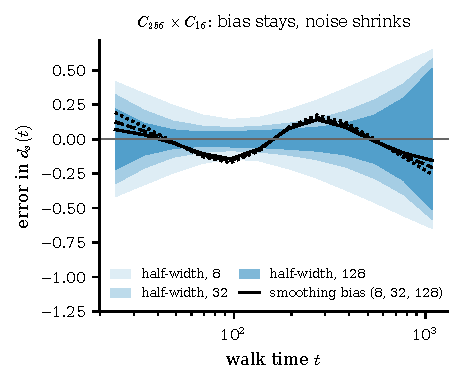
\includegraphics[width=\columnwidth]{figs/fig1a_v8}
\caption{Bias against noise for the smoothing band on $C_{256}\times C_{16}$ (100 datasets per budget). Lines: the smoothing bias $d_{\rm pop}(t)-d(t)$, mean over datasets, at 8 (dotted), 32 (dashed) and 128 (solid) walkers per node. Shading: the median half-width of the 95\% band, drawn about zero. The bias barely moves as walkers are added and the band narrows; at 128 walkers per node the magnitude of the mean bias is larger than the median half-width at $t=68,96,136,192,272$.}
\label{fig:budget}
\end{figure}

\emph{The decline.} To change only the amount of data, we fixed the window of each graph in advance from its exact curve and ran \LQ{} on the 18 graphs with a realised crossover, 200 datasets per graph and budget. Of 3600 datasets per budget 3200 were answered (two graphs have windows shorter than six points). The band covered the exact curve in 1292, 627 and 114 of them: 40.4\% (38.7--42.1), 19.6\% (18.2--21.0) and 3.6\% (2.9--4.3) at 8, 32 and 128 walkers per node. Over the same data the fraction of datasets in which the band declared a change in $d$ rose from 72.1\% to 97.1\% (a change is declared when the band for $d(t_j)-d(t_0)$ lies wholly beyond $\pm0.25$; \SM\ Sec.~\ref{S-sup:bench}): the band became more decisive as it became less often right.

The decline was first seen in exploratory runs. Its ordering was then written down as a prediction and tested on fresh data three times, in the fixed-window run above, in a replication on new seeds with the code frozen (49.6\%, 18.3\%, 4.0\%), and in a holdout on graph sizes used in no earlier run (57.3\%, 26.1\%, 10.0\%). It held each time (Table~\ref{tab:conf}).

\subsection{Why: the bias stays and the noise shrinks}\label{sec:mech}
A smoothing band is centred on a smoothed curve, $d_{\rm pop}(t)$: what the smoother returns when its fitted weights for that dataset, at its bandwidth, are applied to the exact $\ln q$ curve. Its width reflects the noise about $d_{\rm pop}$. Nothing in it accounts for the bias $d_{\rm pop}(t)-d(t)$.

Scored against its own smoothed target, the band is nearly at its nominal level: on the fixed-window data it covered $d_{\rm pop}$ in 94.7\%, 94.3\% and 93.0\% of answered datasets at the three budgets. The loss of coverage is therefore mostly bias. Figure~\ref{fig:budget} shows the two parts on $C_{256}\times C_{16}$. At $t=96$, on the bend, the mean bias is $-0.171$, $-0.156$ and $-0.143$ at the three budgets, while the median half-width falls from 0.143 to 0.084 to 0.057. The cross-validated bandwidth shrinks as the data sharpen, but it runs into the smallest value on the menu, $h=0.7$ (about two grid steps), which is chosen in 62.9\% of datasets at 128 walkers per node. At that bandwidth the smoother applied to the exact returns gives 1.7625 at $t=96$, where the exact value is 1.8960: a bias of $-0.1335$ with no noise at all.

\emph{The standard remedies.} A local-cubic robust bias correction \cite{ccf2018,ccf2022}, run on six of the 18 graphs, lifted coverage to 83.5\%, 66.3\% and 47.5\% at about 1.7 times the width, against 50.0\%, 26.5\% and 2.8\% for \LQ{} on the same six graphs. It reduced the decline and did not remove it. Undersmoothing did less (\SM\ Table~\ref{S-tab:rbc}). Bias-aware bands in the manner of Armstrong and Koles\'ar \cite{ak2018,ak2020} widen the interval by a worst-case bias computed from a bound on the third derivative of $\ln P$. With that bound estimated from the data (\BAC{}) they covered 96.2--97.7\% of answered datasets at fixed windows (Table~\ref{tab:conf}). This is a useful practical band, but its theory assumes a known bound; with a fitted one there is no guarantee, and over all generated datasets, unanswered ones included, it covered 85.3--86.8\% (\SM\ Sec.~\ref{S-sup:e4}).

\section{What positivity buys}\label{sec:pos}
\subsection{Bounds without a bandwidth}\label{sec:e7}
For the lazy walk the eigenvalues $\lambda$ of $S$ lie in $[0,1]$. With $s=-\ln\lambda$,
\begin{equation}
q(t)=\int_{[0,\infty]} e^{-st}\,d\nu(s),\qquad \nu\ge0,
\label{eq:cm}
\end{equation}
with total mass one and mass at least $1/N$ at $s=0$ (the stationary state). The spectral dimension is a ratio of two linear functionals of the same measure, $d(t)=2t\int se^{-st}d\nu/\int e^{-st}d\nu$. The band we call \MLP{} takes a simultaneous confidence box for $q$ at the grid times and reports, at each window time, the smallest and largest $d(t)$ over \emph{all} measures of the form~(\ref{eq:cm}) that fit the box. Each endpoint is a linear-fractional programme, solved as a linear programme (Charnes--Cooper; \SM\ Sec.~\ref{S-sup:e7}). There is no bandwidth, no derivative bound and no sample split, and a window of two points is enough.

With a bootstrap box of nominal level 98.1\%, \MLP{} covered the exact curve in 98.8\% (98.4--99.1) of realised-crossover datasets and 99.8\% (99.6--99.9) of control datasets at 32 walkers per node, and its coverage stayed high across budgets (Table~\ref{tab:conf}: 99.4\%, 98.9\% and 99.1\% in the replication, 99.8\% at all three in the holdout). These bands are computed on a finite grid of atoms for the measure. A continuum outer relaxation was run only on a chosen subset of 1030 datasets, where it covered the exact curve in 1029; the headline coverage belongs to the discretised bands. The level of the box is nominal; details and numerical checks are in \SM\ Sec.~\ref{S-sup:e7}.

\subsection{A crossover test over all admissible measures}\label{sec:nodrop}
The same constraint set answers a sharper question than a band does. Fix a margin, here 0.25, and let $t_0<t_1<\dots$ be the window times. The null hypothesis is that \emph{some} admissible measure shows no drop anywhere,
\begin{equation}
\exists\,\nu\ \text{admissible}:\quad d_\nu(t_j)\ge d_\nu(t_0)-0.25\ \ \forall\,j\ge1 .
\label{eq:null}
\end{equation}
If no such measure exists, every return curve consistent with the data drops by more than the margin somewhere in the window, and the test declares a crossover. For a fixed value of $d(t_0)$ condition~(\ref{eq:null}) is linear in $\nu$, so the null is decided by a one-parameter family of linear programmes. When the null stands, the test returns an explicit no-drop measure that fits the box; the data cannot then decide. The search can also end inconclusive (an unresolved interval, the programme limit, or a solver status), which is not counted as a declaration, and the implementation keeps a numerical guard of 0.005 on the margin (\SM\ Sec.~\ref{S-sup:nodrop}). Simpler tests on the same box are weaker: comparing the band endpoints at two times, or requiring one time $t_j$ to carry the drop for every measure (the joint test).

\subsection{An exact box and a certified level}\label{sec:cp}
Walkers are independent and start uniformly, so the number of returns at a grid time is binomial with success probability $q(t)$. A Clopper--Pearson interval with miss probability $0.05/K$ at each of the $K$ grid times therefore contains all $K$ values of $q$ at once with probability at least 95\%, at any number of walkers and whatever the dependence between times. On that event the true spectral measure is admissible, so a declared drop of more than the 0.25 margin is real. (The margin is not the drop of 0.6 that defines a realised crossover in Sec.~II; the test certifies the smaller drop.) The probability of a false declaration is at most 5\%, in finite samples and with a window chosen from the data, provided the declaration rules out every admissible no-drop measure, on or off the atom grid. The programmes search a finite grid, so this is checked separately, as described at the end of this section. As a check of the simulation, the box contained the exact $q$ at all 28 grid times in 1917 of 2000 datasets on a ring.

\begin{table}[b]
\caption{Crossover tests on the exact Clopper--Pearson box (CONFIRMATORY; not the bootstrap box of \SM\ Table~\ref{S-tab:nodropS}, which uses the same seeds and gives other counts): datasets with a declared drop larger than 0.25, of 100 per row (300 for the controls), by walkers per node. Secant: a log-convexity bound through the box. Endpoint: band endpoints at two times. Joint and Global: Sec.~\ref{sec:nodrop}. Controls: a ring, a 2D torus and a 3D torus (exact drops at most 0.053).}
\label{tab:nodrop}
\begin{ruledtabular}
\begin{tabular}{lccccc}
Graph & Walkers & Secant & Endp. & Joint & Global \\
\hline
$C_{768}\times C_{16}$ & 8 & 0 & 0 & 0 & 1 \\
(2D to 1D) & 32 & 0 & 3 & 5 & 85 \\
 & 128 & 0 & 95 & 95 & 100 \\
$C_{160}\times C_8^2$ & 8 & 0 & 1 & 12 & 37 \\
(3D to 1D) & 32 & 1 & 83 & 100 & 100 \\
 & 128 & 52 & 100 & 100 & 100 \\
Controls & 32 & 0 & 0 & 0 & 0 \\
\end{tabular}
\end{ruledtabular}
\end{table}

Table~\ref{tab:nodrop} gives the result. At 32 walkers per node the global test declared the 2D crossover in 85 of 100 datasets (76.5--91.4), where the joint, endpoint and secant tests on the same exact box declared 5, 3 and 0 (0, 0, 0 on the bootstrap box, \SM\ Table~\ref{S-tab:nodropS}). Across eight graphs (four sizes per family) its power never fell as walkers were added, and it reached 100 of 100 at 512 walkers per node in every one (grid-search results, \SM\ Table~\ref{S-tab:cpmap}; all 2330 of its declarations passed the continuum check below). No drop was declared in 900 datasets from graphs whose exact drop is below the margin: the 300 controls, and 600 from three small products with exact drops of 0.14 to 0.23. The window is chosen from the data, so these drops were recomputed over the window each dataset actually used: the largest is 0.229, and 71 datasets had no window. A longer window could have exceeded the margin (on $C_{39}\times C_8$ one more grid time gives 0.540), but no dataset selected one. The level bound does not tighten with data; what rises is the detection rate, where for the smoothing band more data hurt. With the bootstrap box of Sec.~\ref{sec:e7} the global test had declared 37 of the same 100 two-dimensional datasets at 32 walkers per node, all of them among the 85; the exact box is the narrower of the two. \emph{Pre-registered outcomes.} The level and power bars were fixed in advance and met; three recorded predictions failed: 8 to 20 declarations at 32 walkers per node (85 observed), power from an exact drop of 0.30 (none), and at most three extra declarations from exact low-order constraints (15). The level claim held; the predicted counts did not. The 5\% bound is proven, not measured; it rests on the exact CP box, a certified exclusion of continuum no-drop measures (below) and drops above 0.25, and the null runs cover only 32 and 128 walkers per node.

\emph{From a grid to all measures.} The programmes search measures on a finite grid of atoms, which restricts the null. For every declaration in Table~\ref{tab:nodrop}, 423 in all, we therefore checked that no nonnegative measure, on or off the grid, fits the box without a drop: the dual multipliers of the infeasible programmes were bounded over the whole support $s\in[0,\infty]$ by interval branch and bound. All 423 passed. The multipliers come from a floating-point solver, but the check does not trust them: the dual coefficients, the objective and the bound over the whole support were recomputed from the raw multipliers in 100-bit ball arithmetic (Arb), and every one of the 423 certificates passed, as did those of all 2330 declarations of the power map (\SM\ Sec.~\ref{S-sup:nodrop}). The box endpoints are computed in double precision; for this check each was widened outward (by a relative $2^{-30}$, $2^{-24}$ for ten datasets) and the widening was proven to contain the exact Clopper--Pearson endpoint by a ball-arithmetic bound on the binomial tail, so the chain from counts to declaration is rigorous. All 2330 declarations pass on the widened box.

\section{Limits}\label{sec:limits}\label{sec:rec}
\emph{The finding.} The decline is shown for one smoothing band, with a cross-validated bandwidth, on a fixed time grid, for a lazy walk on product tori; a random-graph run agreed in direction (\SM\ Sec.~\ref{S-sup:rand}). The bias correction is our implementation, run on six graphs, and finer time grids and bandwidths chosen for the derivative were not tested. \emph{The fix.} The certified level needs independent walkers, a uniform start, a lazy walk and a connected graph, and it was run on tori only. The graphs with exact drops just above the margin (0.27 to 0.34) were small, with windows of two to seven points or none, and the test declared nothing on them: its power near the margin, and its level just under the margin with a long window, are untested. The positivity band was scored with a nominal box only. Quantities that are not completely monotone, such as mean-squared displacements, are outside the method. \emph{Interpretation.} A declared drop is a statement about this walk on this finite graph. Equilibration alone depresses $d$, and a claim about geometry needs size scaling and a second operator.

\section*{Pre-registration, data and code}
The plan was committed before the first run, and each later addition before the run it governs. The decline with the budget and the level and power of the exact-box test were scored against bars fixed in advance; the bias analysis, the bias-correction comparison and the coverage of the positivity band are exploratory. The full record of labels, bars, amendments and failed predictions is in \SM\ Sec.~\ref{S-sup:bench} and Table~\ref{S-tab:ledger}. Code, plans with their commit history, stored per-dataset results and a script that regenerates the tables of the analyses in that release from them are public \cite{archive2026}: version 1.1, DOI \texttt{10.5281/zenodo.24520991}, mirrored at {\footnotesize\mbox{\url{github.com/mobluehq-llc/spectral-dimension-coverage}}}. Version 1.1 does not contain the exact-box run of Sec.~\ref{sec:cp} (Table~\ref{tab:nodrop}), which was registered and run after that release; its plan, code, raw rows and result tables will be in version 1.2 of the archive.

\section*{How these results were obtained}
We used blueMonster, a tool developed by MOBLUEHQ, Inc., to generate research topics and brainstorm ideas. The simulation code, the pre-registered plans, the analysis and the text were written with Claude large language models (Anthropic) under the author's direction; repeated rounds of LLM critiques, one of them a red-team round, were obtained from ChatGPT (OpenAI) and, from the fourth round on, Gemini (Google), and the checks they named are identified in the text and the \SM. The numbers in the text were checked against the committed result files. Software, independent verification and a reproducibility spot check are described in \SM\ Sec.~\ref{S-sup:soft}. The author takes responsibility for the content.

The author is an amateur, with no formal training in statistical physics or in statistics and no research publication in either. Much of this work was done while improving MOBLUEHQ's software tools, by using them on a real problem. His inexperience should invite heavy scepticism towards the methods and the claims: errors of a kind a trained researcher would not make are possible, and the checks described here lower that risk without removing it. He welcomes corrections.

\emph{Competing interests.} The author is the founder of MOBLUEHQ, Inc., which develops and intends to sell blueMonster.

\begin{acknowledgments}
The author thanks Dr Franti\v{s}ek Ga\v{s}par for kindly sharing Ref.~\cite{gk2022}, which made the comparison in \SM\ Sec.~\ref{S-sup:gk} possible. Any error in our reading or implementation of that work is the author's.
\end{acknowledgments}


\bibliography{refs}

\end{document}
